\documentclass[12pt]{article}
\usepackage{graphicx}
\usepackage{amssymb}
\usepackage{amsthm}
\usepackage{amsmath}
\usepackage{bm}
\usepackage{fullpage}
\newcommand{\dd}{\displaystyle}
\newcommand{\ZZ}{\mathbb{Z}}
\newcommand{\RR}{\mathbb{R}}
\newcommand{\FF}{\mathbb F}
\newcommand{\LL}{\mathbb L}
\newcommand{\EE}{\mathbb E}
\newcommand{\MM}{\mathbb M}
\newcommand{\KK}{\mathbb K}
\newcommand{\HH}{\mathbb H}
\newcommand{\QQ}{\mathbb Q}
\newcommand{\CC}{\mathbb{C}}
\newcommand{\Pin}{P_{\text{in}}}
\newcommand{\bx}{\mathbf{x}}
\newcommand{\bp}{\mathbf{p}}
\newcommand{\by}{\mathbf{y}}
\newcommand{\cP}{{\cal P}}
\newcommand{\bB}{\mathbf B}
\newcommand{\bM}{\mathbf M}
\newcommand{\bS}{\mathbf S}
\newcommand{\phis}{\varphi}
\newcommand{\barphis}{\overline\phis}
\newcommand{\bmat}{\begin{matrix}}
\newcommand{\emat}{\end{matrix}}
\newcommand{\se}{\text{se}}
\newcommand{\daga}{a^\dagger}
\newcommand{\devides}{\bigl |}
\newcommand{\eval}{\biggl |}
\newcommand{\ybar}{\overline y}
\newcommand{\bWhat}{\hat{\mathbf W}}
\newcommand{\bW}{\mathbf W}
\newcommand{\bz}{\mathbf z}
\newcommand{\bs}{\mathbf s}
\newcommand{\rightas}{\stackrel{a.s.}{\rightarrow}}
\newcommand{\rightp}{\stackrel{p}{\rightarrow}}
\newcommand{\rightd}{\stackrel{d}{\rightarrow}}
\newcommand{\bI}{\mathbf I}
\newcommand{\barB}{{\overline B}}
\newcommand{\barC}{{\overline C}}
\newcommand{\pbar}{{\overline p}}
\newcommand{\bbar}{{\overline b}}
\newcommand{\mubar}{{\overline \mu}}
\newcommand{\var}{{\text{var}}}
\newcommand{\cov}{{\text{cov}}}
\newtheorem{lemma}{Lemma}
\newtheorem{proposition}{Proposition}
\title{Characterizing the Ergodic Distribution with Risky Debt}
\date{}

\begin{document}
\maketitle
\section{The Problem}
We wish to solve the following optimal planning problem with risky debt.  We assume that there are $s = 1,\ldots,S$ aggregate states of the world with Markov transition matrix $\Pi$.  For now we assume that the Markov transition matrix is i.i.d.  Each state of the world $s$ is associated with the exogenous government expenditure $g_s$ and a payoff for government debt $p_s$.  With the normalization $\EE p = 1$.  The planning problem can then be written recursively as 
\[
	V(b) = \max_{c(s),l(s),b'(s)}\sum_s \Pi(s)\left[ c(s) - \frac{l(s)^{1+\gamma}}{1+\gamma}+ \beta V(b'(s)) \right]
\]subject to the constraints
\begin{subequations}
\begin{align}\label{eq.imp}
	c(s) - l(s)^{1+\gamma}  + b'(s)  = \frac{p_s b}{\beta}\\
	c(s) + g_s  \leq l(s)\label{eq.res}
\end{align}
\end{subequations} Note that equation \eqref{eq.imp} being an equality constraint implies that we are ruling out transfers for now.  We will also assume that if $s'\neq s''$ then $p_{s'}\neq p_{s''}$.
\subsection{Debt Limits}
In addition to constraints in equations (\ref{eq.imp}-\ref{eq.res}) we place upper and lower bounds on the level of government debt.  The lower limit to government debt is chosen to be the natural debt limit.  As noted before the largest tax rate the government will implement is $\tau = \frac{\gamma}{1+\gamma}$ (as any higher tax rate will reduce government revenue).  This leads to the natural debt limit being 
\begin{equation}
	\overline b = \min_{s}\left(\frac{p_s}{\beta}-1\right)^{-1}\left(\left(\frac1{1+\gamma}\right)^\frac1\gamma\frac\gamma{1+\gamma} - g_s\right)
\end{equation}

For now we will choose an arbitrary lower limit on government debt $\underline b$
\subsection{First Order Conditions}
We have already shown that under an appropriate change of variables the problem is concave so $V(b)$ is a concave function.  Letting $\underline \lambda$ being the Lagrange multiplier on the constraint $\underline b \leq b'(s)$ the first order conditions associated with our problem are
\begin{align}
	1-\mu(s)-\xi(s) = 0\label{eq.foc1}\\
	\xi(s) +((1+\gamma)\mu(s)-1)l(s)^\gamma  = 0\label{eq.foc2}\\
	\beta V'(b(s)) - \mu(s) +\underline \lambda(s) = 0\label{eq.foc3}
\end{align}Combining with the envelope condition 
\[
	V'(b) = \sum_s\Pi(s)p_s\mu(s)/\beta
\] we have the martingale condition
\begin{equation}\label{eq.mart}
	\mu_t = \EE_t p_{t+1}\mu_{t+1}+\underline{\lambda}_t
\end{equation}  The inequality in the resource constraint implies that $\xi(s)\geq 0$ implying that $\mu(s) \leq 1$.  With some minor algebra algebra we obtain
\[
	l(s)^\gamma = \frac{\mu(s)-1}{(1+\gamma)\mu(s) - 1} = 1-\tau(\mu(s))
\]implying the relationship between tax rate $\tau$ and multiplier $\mu$ given by
\begin{equation}\label{eq.tau}
	\tau(\mu) = \frac{\gamma\mu}{(1+\gamma)\mu-1}
\end{equation}  We quickly see that $\lim_{\mu\rightarrow \frac{1}{1+\gamma}} \tau(\mu) = -\infty$ and $\lim_{\mu\rightarrow-\infty} \tau(\mu) = \frac{\gamma}{1+\gamma}$ implying that $\mu(s)\in (-\infty,\frac1{1+\gamma}]$ so $\xi(s) > 0$ for all $b$ and the resource constraint, equation \eqref{eq.res}, can be assumed to hold with strict equality.

We should also note that the labor choice is entirely determined by the multiplier on the implementability constraint
\begin{equation}\label{eq.l_mu}
	l(\mu) = \left(\frac{\mu-1}{(1+\gamma)\mu - 1}\right)^\frac1\gamma
\end{equation} and consumption is then
\[
	c_s(\mu) = l(\mu) - g_s
\]  The government surplus 
\begin{equation}\label{eq.S}
	S_s(\mu) = c(\mu) -l(\mu)^{1+\gamma}= l(\mu)-l(\mu)^{1+\gamma} - g_s
\end{equation} can be shown to be decreasing in $\mu$ for $\mu\in(-\infty,\frac1{1+\gamma}]$
\subsection{Drift Away from Bonds}\label{sec.drift}
From Mike's notes we know that under the correct change of variables the problem can be written as maximizing a linear objective function over a convex set.  He is then able to show that the value function $V(b)$ is concave and the policy functions are continuous.  In this first section we will show that there exists $b_1$, and if $p$ is sufficiently volatile a $b_2$, such that if $b_t\leq b_1$ then 
\[
	\mu_t \geq \EE_t \mu_{t+1}
\] and if $b_t \geq b_2$ then
\[
	\mu_t \leq \EE_t \mu_{t+1}.
\]  Recall that $b$ is decreasing in $\mu$, so this implies that if $b_t$ is low (large) enough then there will exist a drift away from the lower (upper) limit of government debt.
\begin{lemma}  Let $\mu(b,s)$ be the optimal policy function for the Lagrange multiplier $\mu(s)$.  If $p_{s'} > p_{s''}$ then there exists a $b^*_{s',s''}$ such that for all $b < (>) \; b_{1,s',s''}$ we have $\mu(b,s') > (<) \;\mu(b,s'')$.  If $\underline b < b^*_{s',s''} < \overline b$ then $\mu(b^*_{s',s''},s') = \mu(b^*_{s',s''},s'')$.
\label{lem.order}
\end{lemma}
\begin{proof} 
Suppose that $\mu(b,s')\leq \mu(b,s'')$.  Subtracting the implementability for $s''$ from the implementability constraint for $s'$ we have 
\begin{align*}
	\frac{p_{s'}-p_{s''}}{\beta}b &= S_{s'}(\mu(b,s'))-S_{s''}(\mu(b,s'')) + b'(b,s')-b'(b,s'')\\
						&\geq S_{s'}(\mu(b,s')) -S_{s''}(\mu(b,s')) + b'(b,s')-b'(b,s'')\\
						&\geq  S_{s'}(\mu(b,s')) -S_{s''}(\mu(b,s')) = g_{s''}-g_{s'}
\end{align*}  We get the first inequality from noting that $S_s(\mu')\geq S_s(\mu'')$ if $\mu' \leq \mu''$.  We obtain the second inequality by noting that $\mu(b,s')\leq \mu(b,s'')$ implies $b'(b,s')\leq b'(b,s'')$ (which comes directly from equation \eqref{eq.foc3} and concavity of $V$).  Thus, $\mu(b,s')\leq \mu(b,s'')$ implies that 
\[
	b \geq \frac{\beta(g_{s''}-g_{s'})}{p_{s'}-p_{s''}} = b^*_{s',s''}
\]The converse of this statement is that if $b<b^*_{s',s''}$ then $\mu(b,s') > \mu(b,s'')$.  The reverse statement that $\mu(b,s') \geq \mu(b,s'')$ implies $b \leq b^*_{s,s'}$ follows by symmetry.   Again, the converse implies that if $b > b^*_{s',s''}$ then $\mu(b,s') < \mu(b,s'')$.    Finally, if $\underline b < b^*_{s',s''} <\overline b$ then continuity of the policy functions implies that there must exist a root of $\mu(b,s')-\mu(b,s'')$ and that root can only be at $b^*_{s',s''}$.
\end{proof}

With Lemma \ref{lem.order} we can order the policy functions $\mu(b,\cdot)$ for particular regions of the state space.  Take $b_1$ to be
\[
	b_1 = \min\left\{b^*_{s',s''}\right\}
\] and WLOG choose $\underline b < b_1$.  For all $b < b_1$ we have shown that $p_s > p_{s'}$ implies that $\mu(b,s) > \mu(b,s')$.  By decomposing $\EE \mu_{t+1}p_{t+1}$ in equation \eqref{eq.mart}, we obtain (using $\EE_t p_{t+1} = 1$)
\begin{equation}
	\mu_t = \EE\mu_{t+1} +\cov_t(\mu_{t+1},p_{t+1}) + \underline \lambda_t
\end{equation}Our analysis has just shown that for $b_t < b_1$ we have $\cov_t (\mu_{t+1},p_{t+1})  >0$ so 
\[
	\mu_t > \EE_t\mu_{t+1}.
\]  If $p$ is sufficiently volatile:
\[
	p_{s'} - p_{s''} > \frac{\beta(g_{s''}-g_{s'})}{\overline b}
\] then 
\[
	b_2 = \max\left\{b^*_{s',s''}\right\} <\overline b
\] and through a similar argument  we can conclude that $\cov_t(\mu_{t+1},p_{t+1}) < 0$ 
\[
	\mu_t < \EE_t \mu_{t+1}
\] for $b_t > b_2$ (note $b_t >\underline b$ implies $\underline \lambda_t =0$) which gives us a drift away from the upper-bound. 
\subsection{Steady States}  Generically there do not exist steady state for arbitrary $p$ if there are more than 2 government expenditure states.  There do exist payoff structures where a steady state does exist.  Specifically let
\[
	p^\alpha_s = 1 + \alpha(g_s - \EE g)
\]It is straightforward to show that $b^*_{s',s} = \frac\beta\alpha$, which implies all policy rules cross at the same level of government debt.  This in turn implies that $b'(\frac\beta\alpha,s) = \frac\beta\alpha$ for all $s$, and thus, that $\frac\beta\alpha$ is a steady state.  Using the results of the previous section, we have that $b_1 = b_2 = \frac\beta\alpha$, implying that $\mu_t < (>) \EE_t\mu_{t+1}$ for $b_t  < (>) \frac\beta\alpha$.  Extending our 2-state result we then quickly obtain that the economy $b_t \rightarrow \frac\beta\alpha$ with probability 1.

Now suppose we have a sequence $p^i$ such that $\lim_{i\rightarrow\infty} p^i_s = p^\alpha_s$ for all $s$.  If we let $b_1(p)$ be the largest $b_1$ for a given $p$ such that for all $b_t < b_1$ we have $\mu_t > \EE_t\mu_{t+1}$, and similarly for $b_2(p)$.  A straightforward application of our formulas in section \ref{sec.drift} implies that $\lim_{i\rightarrow \infty} b_1(p^i) = \lim_{i\rightarrow\infty} b_2(p^i) = \frac\beta\alpha$.
\subsection{Ergodic Distribution}
We can also characterize the ergodic distribution using our numeric code.  Roughly the algorithm proceeds as follows:
\begin{enumerate}
	\item Compute the policy rules numerically
	\item Divide $[\underline b,\overline b]$ into a grid with $N$ bins.  I used $N = 2000$ with greater weight placed on areas with high density.
	\item  Construct a transition matrix $T$ assuming that mass is evenly distributed in each bin and policy rules are locally linear. (Using a sparse matrix its is possible to choose very large $N$)
	\item  Find a distribution $\mu$ such that $\mu = T\mu$, this is done by guessing a $\mu_0$ and iterating on $\mu_{t+1} = T\mu_t$ until $\mu_{t+1}\approx\mu_t$
\end{enumerate}

We start out by calibrating the economy as follows:  $\gamma$ we set at $2$, productivity was set to $1$, $g$ was set to follow a 3-state iid process placing equal probability weights on $0.15,0.17,0.19$.  We choose $p$ such that the steady state level of debt is $1.1$ then
\[
	p = (p_1,p_2,p_3) = (1.01727273,  1.,  0.98272727).
\]  I then let $p_2$ vary from $p_1$ to $p_3$ an plotted the resulting ergodic distributions in Figure \ref{fig.erg_dist} below:
\begin{figure}[ht]
	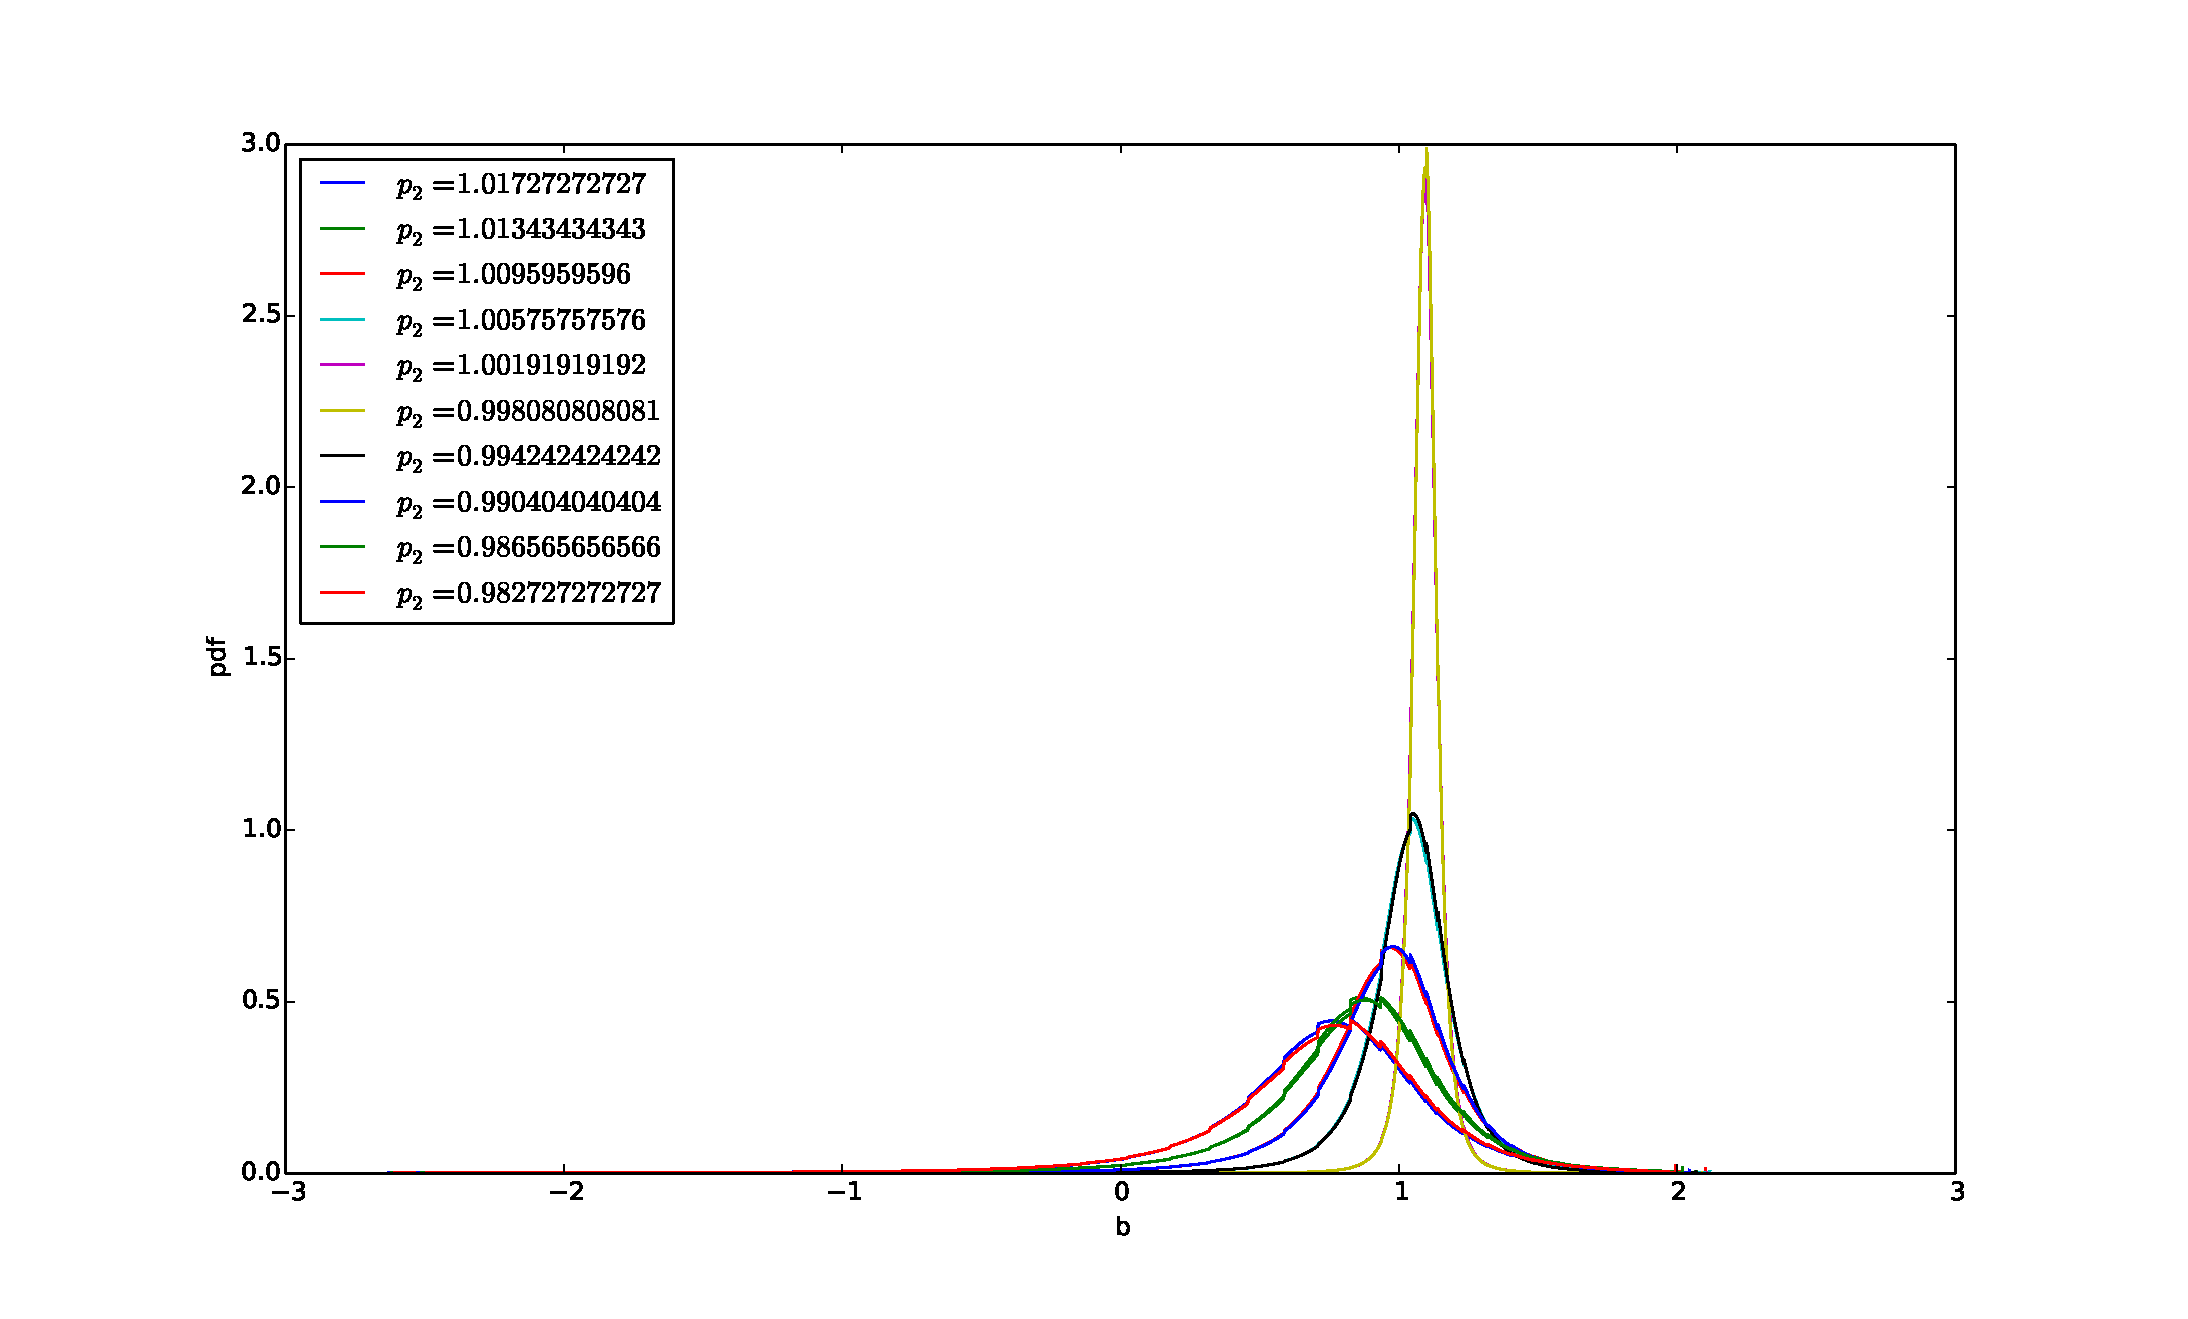
\includegraphics[width=\textwidth]{Images/ergodic_dist.eps}
	\caption{Ergodic distributions as payoff is state 2 is varied.\label{fig.erg_dist}}
\end{figure}

We see several features from this experiment.  First the ergodic distribution becomes tighter and tighter as $p_2$ approaches 1.  Second, moving $p_2$ away from 1 in either direction has approximately the same affect on the ergodic distribution.  As $p_2$ approaches $p_1$ or $p_3$ the ergodic distribution becomes wider and the average debt decreases.
\subsection{Notes}These are some notes that I haven't fleshed out yet:
\begin{itemize}
	\item  Note that if $p_s > p_{s'}$ when $g_s > g_{s'}$ then both $b_1$ and $b_2$ will be greater than zero, and the opposite for for $p_s < p_{s'}$.
	\item  Essentially there are two key aspects of $p$ that matter.  How does $p$ correlate with $g$ and what is the variance of $p$.  
	\begin{itemize}
	\item The more correlated $p$ is with $g$ the tighter the ergodic distribution
	\item  The greater the variation  in $p$ the closer the ergodic distribution will be to 0.
	\item  Perfect correlation implies a steady state with sign of correlation determining if the government holds debt or assets.
	\end{itemize}
	\item  This gives us a good intuition for what we will expect to happen if $p$ is uncorrelated with $g$. Assuming that $p$ has some variation we expect the ergodic distribution to be centered around $0$ and to become tighter as variance of $p$ increases.
\end{itemize}
\section{Linearization}
The first order conditions for a planning problem given portfolio $p_s$ are given by
\begin{align*}
	\frac{b p_s}{\beta \EE p}= S(\mu'(s),s) + b'(s)\\
	V'(b) = \frac{\EE p \mu'}{\EE p}\\
	\mu'(s) = V'(b'(s))
\end{align*} where $S(\mu,s)$ is the government surplus in state $s$ given by
\[
	S(\mu,s) = (1-\tau(\mu))^\frac1\gamma \tau(\mu)-g(s) = I(\mu) - g(s)
\]where
\[
	\tau(\mu) =\frac{\gamma\mu}{(1+\gamma)\mu-1}
\]We note that $V'(b)$ is one-to-one, so we can re-characterize these equations as searching for a function $b(\mu)$ such that the following two equations can be solved for all $\mu$.
\begin{align}\label{eq.lin_imp}
	\frac{b(\mu)p_s}{\beta \EE p} = I(\mu'(s)) - g(s) +b(\mu'(s))\\
	\mu = \frac{\EE\mu' p}{\EE p}\label{eq.lin_mart}
\end{align}  This defines, implicitly, a function $b(\mu; p)$ .  For a given $\overline \mu$ define 
\[
	\overline b = \frac{\beta}{1-\beta}\left( I(\overline\mu) - \overline g\right)
\]where $\overline g = \EE g$ and $\overline p$ as 
\[
	\overline p_s = 1+ \frac\beta{\overline b}(g_s - \overline g)
\]  As noted before $b(\overline\mu;\overline p) = \overline b$ solves the the system of equations (\ref{eq.lin_imp}-\ref{eq.lin_mart}) for $\mu'(s) = \overline \mu$.  We can linearize around this steady state with respect to both $\mu$ and $p$.  Differentiating equation \eqref{eq.lin_imp} with respect to $\mu$ around $(\overline \mu,\overline p)$ we obtain
\[
	\frac{\pbar_s}{\beta}\frac{\partial b}{\partial \mu} = \left[I'(\mubar)+\frac{\partial b}{\partial \mu}\right]\frac{\partial \mu'(s)}{\partial \mu}.
\]Differentiating equation \eqref{eq.lin_mart} with respect to $\mu$ we obtain
\[
	1 = \sum_{s'} \Pi_s \overline p_s \frac{\partial \mu'(s)}{\partial \mu}
\]combining these two equations we see that 
\[
	\frac1\beta\left(\sum_s\Pi_s\pbar_s^2\right)\frac{\partial b}{\partial \mu} = I'(\mubar) + \frac{\partial b}{\partial \mu}
\]Noting that $\EE\overline p^2 = 1 + \frac{\beta^2}{\bbar^2}\sigma^2_g$ we obtain
\begin{equation}
	\frac{\partial b}{\partial \mu} = \frac{I'(\mubar)}{\frac{\beta}{\bbar^2}\sigma_g^2 +\frac{1-\beta}{\beta}} < 0
\end{equation}as $I'(\mubar) < 0$.  We then have directly that 
\begin{equation}
	\frac{\partial \mu'(s)}{\partial \mu} = \frac{\overline p_s}{\frac{\beta^2}{\overline b^2}\sigma^2_g +1} = \frac{\pbar_s}{\EE\pbar^2}
\end{equation}  We can perform the same procedure for $p_s$.  Differentiating equation \eqref{eq.lin_imp} with respect to $p_s$ we around $(\mubar,\pbar)$ we obtain
\begin{equation}\label{eq.dimp_dps}
\frac{\pbar_{s'}}{\beta}\frac{\partial b}{\partial p_s} + 1_{s,s'}\frac{\bbar}{\beta} - \frac{\Pi_s\bbar\pbar_{s'}}{\beta} = \left[I'(\mubar) + \frac{\partial b}{\partial \mu}\right]\frac{\partial \mu'(s')}{\partial p_s}
\end{equation} Here $1_{s,s'}$ is $1$ if $s = s'$ and zero otherwise.  Differentiating equation \eqref{eq.lin_mart} with respect to $p_s$ we obtain
\[
	0 = \Pi_s\mubar - \Pi_s\mubar + \sum_{s'} \Pi_{s'}\pbar_s\frac{\partial \mu'(s')}{\partial p_s} =  \sum_{s'} \Pi_{s'}\pbar_s\frac{\partial \mu'(s')}{\partial p_s}
\]  Again we can combine these two equations to give us
\[
	\frac{\EE\pbar^2}{\beta}\frac{\partial b}{\partial p_s} + \frac{\Pi_s\bbar}{\beta}(\pbar_s-\EE\pbar^2) = 0
\] or
\begin{equation}
	\frac{\partial b}{\partial p_s} = \Pi_s\bbar \frac{\EE\pbar^2-\pbar_s}{\EE\pbar^2}
\end{equation}Going back to equation \eqref{eq.dimp_dps} we have
\begin{equation}
	\frac{\partial \mu'(s')}{\partial p_s} = \frac{\bbar}{\beta\left[I '(\mubar) + \frac{\partial b}{\partial \mu}\right]}\left(1_{s,s'}-\frac{\Pi_s\pbar_s\pbar_{s'}}{\EE\pbar^2}\right)
\end{equation}
\subsection{Ergodic Distribution of the Linearized System}
The linearized system for $\mu$ now follows
\[
	\hat \mu_{t+1} = B \hat\mu_t + C
\]  where $B$ and $C$ are both random with means $\barB$ and $\barC$, and variances $\sigma_B^2$ and $\sigma_C^2$ .  Suppose that $\hat\mu$ is distributed according to the ergodic distribution of this linear system with mean $\EE\hat\mu$ and variance $\sigma^2_\mu$.  Since 
\[
	B\hat\mu +C
\]has the same distribution we can compute the mean of this distribution as
\[
\begin{split}
	\EE\hat\mu &= \EE\left[ B\hat\mu+C\right]\\
			  &= \EE\left[\EE_{\hat\mu}\left[B\hat\mu+C\right]\right]\\
			  &= \EE\left[\barB\hat\mu +\barC\right]\\
			  &=\barB\EE\hat\mu+\barC
\end{split}
\]solving for $\EE\hat\mu$ we get
\begin{equation}
	\EE\hat\mu = \frac{\barC}{1-\barB}
\end{equation}For the variance $\sigma^2_{\hat\mu}$ we know that 
\[
	\sigma^2_{\hat\mu} = \var(B\hat\mu+C) = \var(B\hat\mu) + \sigma_C^2 + 2\cov(B\hat\mu,C)
\]Computing the variance of $B\hat \mu$ we have
\[
\begin{split}
	\var(B\hat\mu) &=\EE\left[(B\hat\mu - \barB\EE\hat\mu)^2\right]\\
			       &=\EE\left[(B\hat\mu-\barB\hat\mu +\barB\hat\mu -\barB\EE\hat\mu)^2\right]\\
			      &=\EE\left[\EE_{\hat\mu}\left[(B-\barB)^2\hat\mu^2 +2(B-\barB)(\hat\mu-\EE\hat\mu)\barB\EE\hat\mu + (\hat\mu-\EE\hat\mu)^2\bar B^2\right]\right]\\
			&=\EE\left[\sigma_B^2\hat\mu^2 +(\hat\mu-\EE\hat\mu)^2\barB\right]\\
			& = \sigma_B^2(\sigma_{\hat\mu}^2+(\EE\hat\mu)^2) + \sigma_{\hat\mu}^2\barB^2
\end{split}
\]while for the covariance of $B\hat\mu$ and $C$
\[
	\cov(B\hat\mu,C) = \sigma_{BC}\EE\hat\mu
\]Putting this all together we have
\begin{equation}
	\sigma_{\hat\mu}^2 = \frac{\sigma_B^2(\EE\hat\mu)^2 + \sigma_{BC}\EE\hat\mu + \sigma_C^2}{1-\barB^2-\sigma_B^2}
\end{equation}
\subsection{What is the best $\pbar$}
We want to study the properties of the ergodic distribution of an economy with payoff structure $ p_s$, normalized so that $\EE p = 1$.  The immediate question to ask is where we should linearize around?  The natural answer is to choose $\mubar$ so as to minimize 
\[
\| p-\pbar(\mubar)\|^2 = \sum_{s'}\Pi_{s'}( p_{s'}-\pbar(\mubar)_{s'})^2.
\]That is to choose $\mubar$ so as to minimize the variance of the difference between $ p$ and the set of steady state payoffs.  We shall see how this is the ``best'' choice by another metric.  The first order condition for this linearization gives us 
\[
	2\sum_{s'}\Pi_s'( p_{s'}-\pbar(\mubar)_{s'}) \pbar'(\mubar)_{s'} = 0
\]as noted before 
\[
	\pbar(\mubar)_s =  1 -\frac{\beta}{\bbar(\mubar)}\left(g_s - \EE g\right)
\]thus
\[
	\pbar'(\mubar) \propto \pbar(\mubar)-1
\]Thus we can see the the optimal choice of $\mubar$ is equivalent to choosing $\mubar$ such that 
\begin{equation}
	\begin{split}
		0 &= \sum_{s'}\Pi_{s'}( p_{s'} - \pbar(\mubar)_{s'})(\pbar(\mubar)_{s'}-1)\\
		&= -\sum_{s'}\Pi_{s'}( p_{s'}-\pbar(\mubar)_{s'}) + \sum_{s'}\Pi_{s'}( p_{s'}-\pbar(\mubar)_{s'})\pbar(\mubar)_{s'}\\
		&= \sum_{s'}\Pi_{s'}( p_{s'}-\pbar(\mubar)_{s'})\pbar(\mubar)_{s'}\\
		&=\EE\left[( p-\pbar(\mubar))\pbar(\mubar)\right]
	\end{split}
\end{equation}  Using this $\pbar$ and $\mubar$ we have that $C$ for our linearized system is
\[
	C_{s'} = \sum_s\left\{\frac{\bbar}{\beta\left[I'(\mubar)+\frac{\partial b}{\partial\mu}\right]}\left(1_{s,s'}-\frac{\Pi_s \pbar_s\pbar_{s'}}{\EE\pbar^2}\right)({p}_s-\pbar_s) \right\}
\]Taking expectations we have that 
\begin{equation}
\begin{split}
	\barC &= \sum_s\left\{\frac{\bbar}{\beta\left[I'(\mubar)+\frac{\partial b}{\partial\mu}\right]}\left(\Pi_s - \frac{\Pi_s\pbar_s}{\EE\pbar^2}\right)( p_s-\pbar_s)\right\}\\
	&=\frac{\bbar}{\beta\left[I'(\mubar)+\frac{\partial b}{\partial\mu}\right]}\left(\EE( p-\pbar) -\frac{\EE\left[( p-\pbar)\pbar\right]}{\EE\pbar^2}\right)\\
	&= 0 
\end{split}
\end{equation}  Thus the linearized system will have the same mean for $\mu$, $\mubar$, as the closest approximating steady state payoff structure.

We can also compute the variance of the ergodic distribution for $\mu$.  Note 
\[
\begin{split}
	C_{s'} &= \sum_s\left\{\frac{\bbar}{\beta\left[I'(\mubar)+\frac{\partial b}{\partial\mu}\right]}\left(1_{s,s'}-\frac{\Pi_s \pbar_s\pbar_{s'}}{\EE\pbar^2}\right)({p}_s-\pbar_s) \right\}\\
		 &=\frac{\bbar}{\beta\left[I'(\mubar)+\frac{\partial b}{\partial\mu}\right]}\left( p_{s'}-\pbar_{s'} -\pbar_{s'}\frac{\sum_s\Pi_s\pbar_s( p_s-\pbar_s)}{\EE\pbar^2}\right)\\
		&= \frac{\bbar}{\beta\left[I'(\mubar)+\frac{\partial b}{\partial\mu}\right]}( p_{s'}-\pbar_{s})
\end{split}
\]  As noted before
\[
	\sigma_{\mu}^2 = \frac{\bbar^2}{\beta^2\left[I'(\mubar)+\frac{\partial b}{\partial\mu}\right]^2\left(1-\barB^2-\sigma_B^2\right)}\| p-\pbar\|^2
\]  The variance of government debt in the linearized system is 
\[
	\sigma_b^2 = \frac{\bbar^2\left(\frac{\partial b}{\partial\mu}\right)^2}{\beta^2\left[I'(\mubar)+\frac{\partial b}{\partial\mu}\right]^2\left(1-\barB^2-\sigma_B^2\right)}\| p-\pbar\|^2
\]  This can be simplified using the following expressions: 
\[
	I'(\mubar)+\frac{\partial b}{\partial \mu} = \frac{\EE\pbar^2}{\beta}\frac{\partial b}{\partial\mu},
\]
\[
	\barB = \frac{1}{\EE\pbar^2}
\]and
\[
	\sigma_B^2 = \frac{\var(\pbar)}{(\EE\pbar^2)^2}
\] to
\begin{equation}
	\sigma^2_b = \frac{\bbar^2}{\EE\pbar^2\var(\pbar)}\|p-\pbar\|^2
\end{equation}Noting that $\EE\pbar^2 = 1 +\var(\pbar) > 1$, we have immediately that up to first order the relative spread of debt is bounded by
\begin{equation}
	\frac{\sigma_b}{\bbar} \leq \sqrt\frac{\|p-\pbar\|^2}{\var(\pbar)}
\end{equation}  Thus as $p$ approaches a the steady state payoff vector the ergodic distribution becomes degenerate.
\subsection{Intuition}
In incomplete markets fluctuations in the marginal value of debt come from an inability to perfectly insure against fluctuations in government expenditure.  We've seen that when the payoff vector is not constant the planner can use the level of debt to insure against fluctuations in government expenditure.  If the payoff vector is perfectly correlated with government expenditure then there will exist a level of debt where the government has completely insured against all fluctuations to government expenditure with fluctuations in payoffs to government debt.  If the payoff vector $p$ is not perfectly correlated then we can decompose the payoff vector in to two components: 
\[
	p = \hat p + \bar p
\]where $\bar p$ is perfectly correlated with $g$ and $\hat p$ is orthogonal to $g$.  The payoff vector $\pbar$ is associated with a steady state level of debt
\[
	\bbar^2 = -\frac{\beta^2\sigma_g^2}{\cov(p,g)}
\]The variance of $g$ relative to the variance of $p$ in the direction of $g$ determine the ergodic level of debt up of the  first order approximation.  If the government enters the period with debt $b_t$ we can write it's budget constraint as follows
\[
	\frac{\hat p_s b_t}{\beta} + \frac{\pbar_s b_t}{\beta} + g_s = I(\mu'(s)) + b(\mu'(s))
\]When $b_t = \bbar$ the $\frac{\pbar_s b_t}{\beta} + g_s$ term is constant thus all fluctuations in the budget constraint come from $\frac{\hat p_s \bbar}{\beta}$.  This why variance steady state debt of the linear system is proportional to $\bbar^2\|\hat p\|^2$.

\subsection{Accuracy}
We can test the accuracy of the linearized policy rules by comparing the ergodic distributions of the two systems.  In this case we solved a 3 period model where $g$ is iid taking values $0.15$, $0.17$ and $0.19$ with equal probability.   $\pbar$ was choses such that $\bbar = 1.$ and $\hat p$ was chosen to be in the directions $(1,-2,1)$, i.e. making sure $\hat p \cdot g = 0$.  We then solved the system for 
\[
	\sqrt\frac{\var (\hat p)}{\var (\pbar)}
\]taking values $0.25$, $0.5$, and $0.75$.  We then plot the ergodic distribution of both the global and linearized policy rules for these economies in Figure \ref{fig.erg_plot}.
\begin{figure}[ht]
	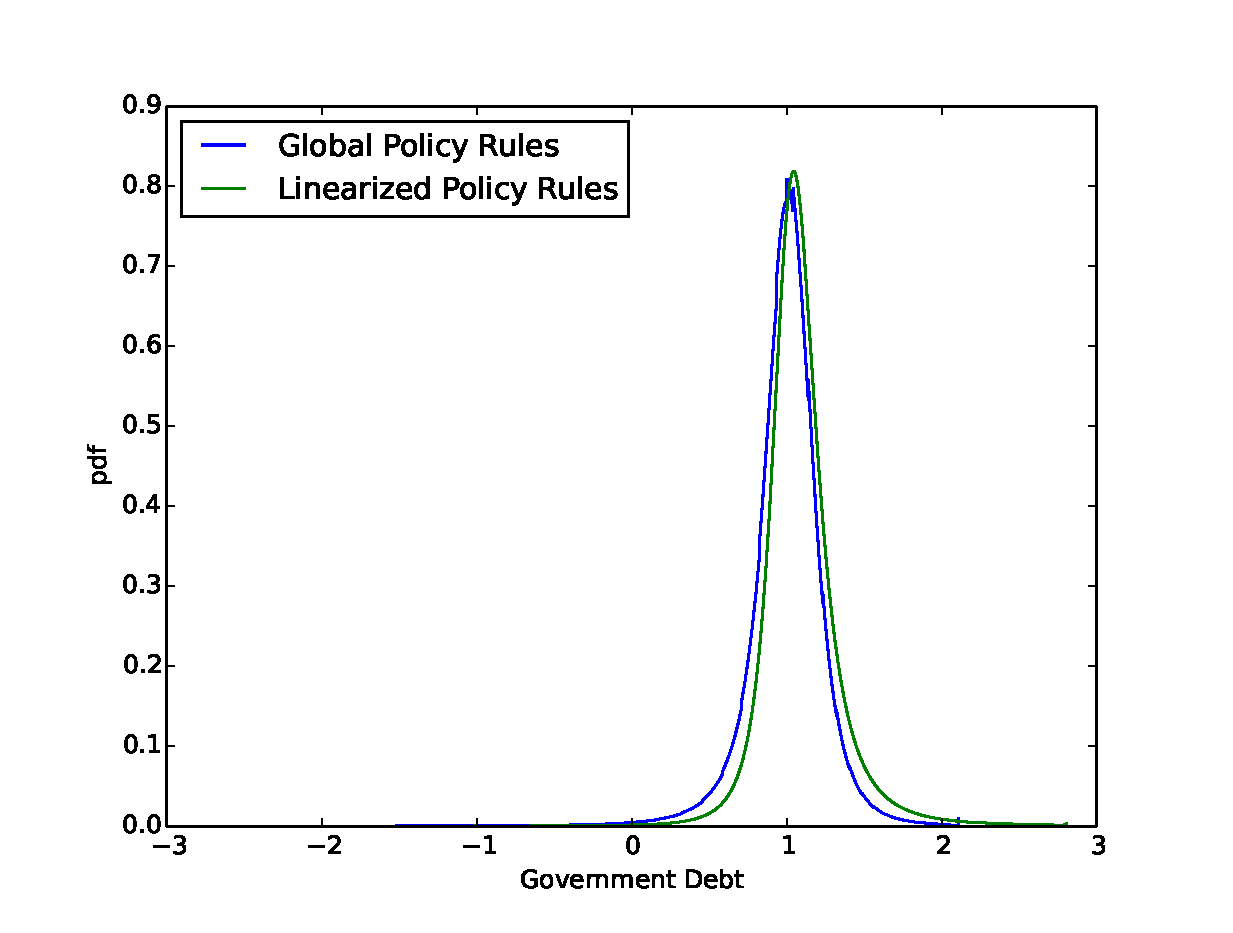
\includegraphics[width=3.5in]{Images/erg1.eps}
	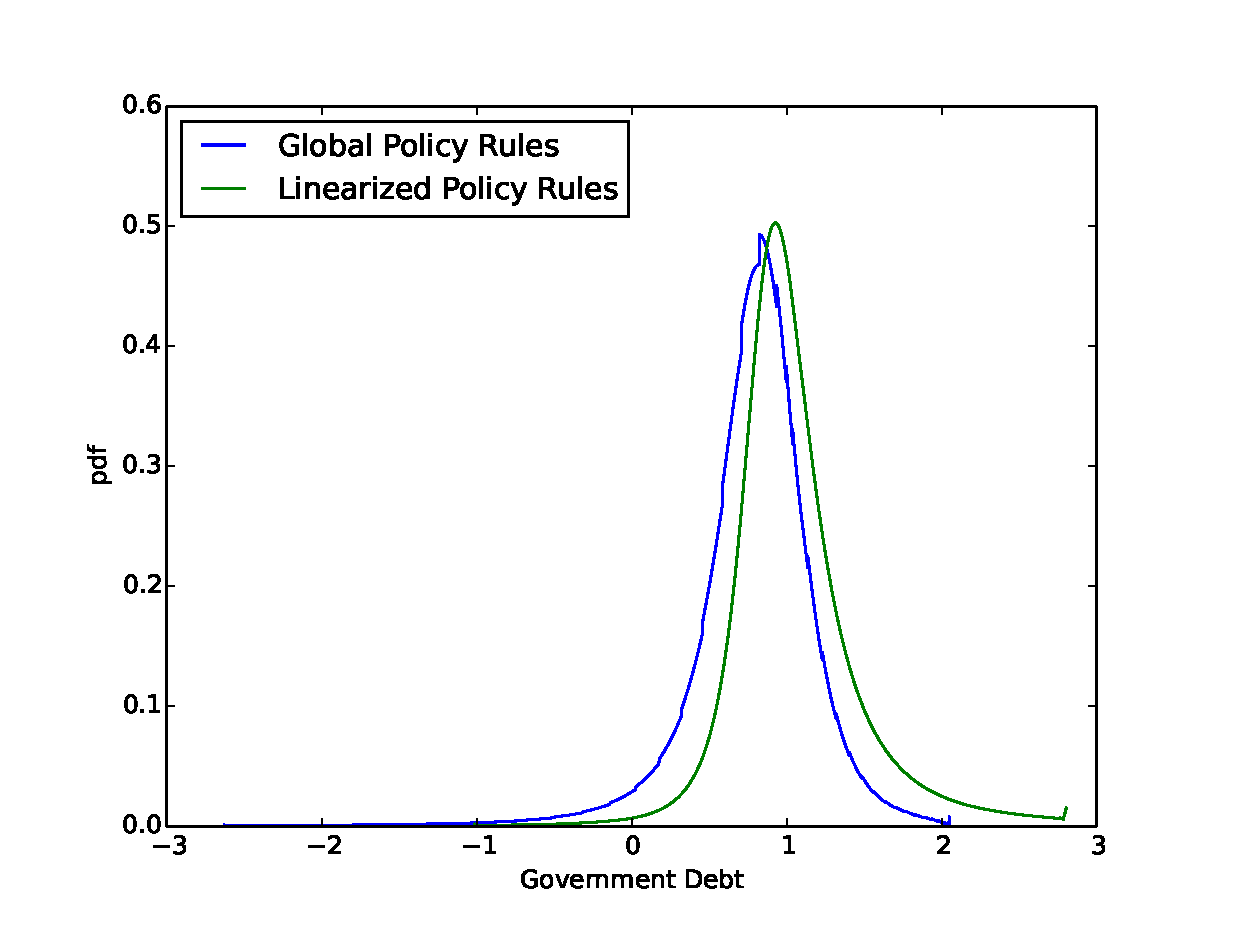
\includegraphics[width=3.5in]{Images/erg2.eps}
	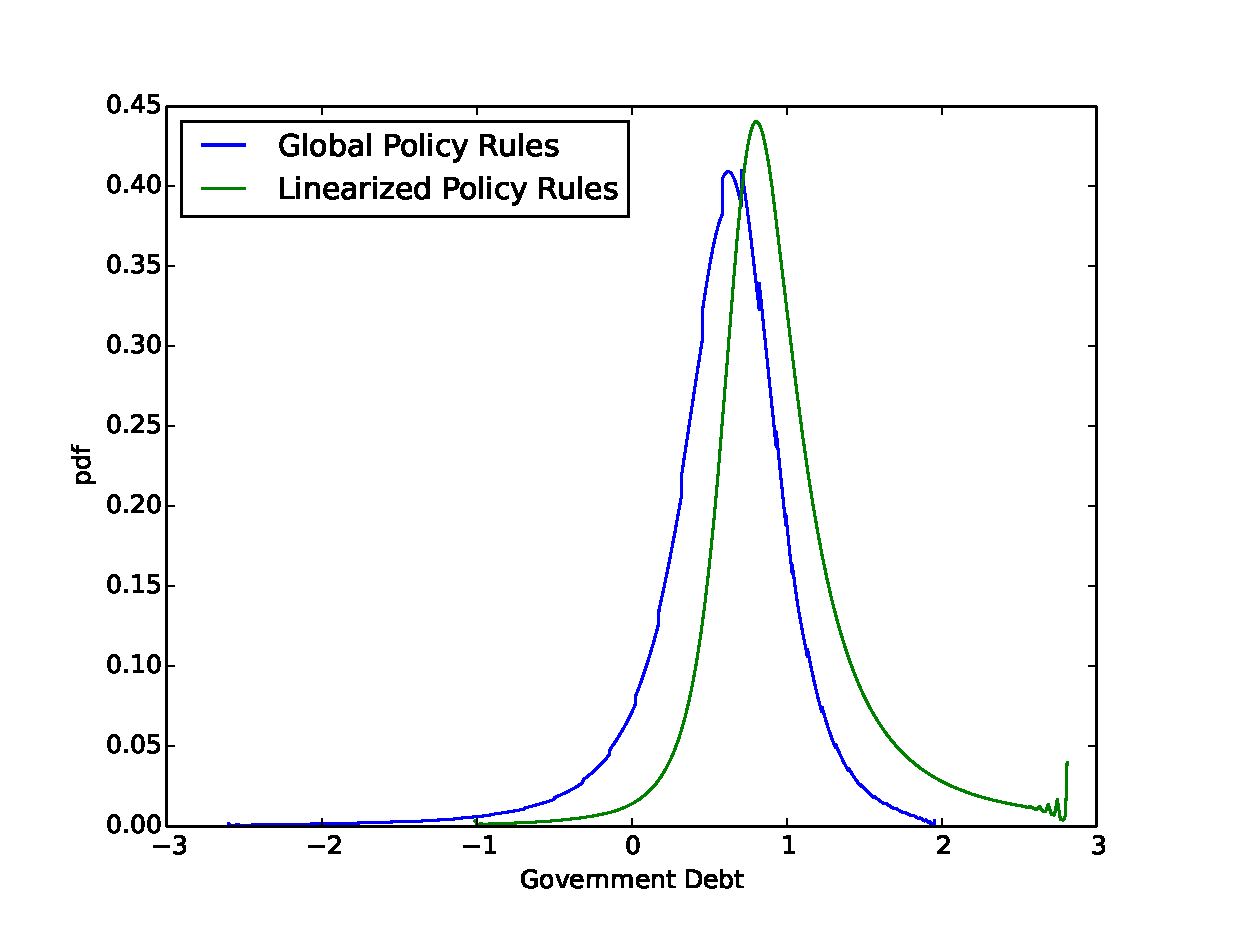
\includegraphics[width=3.5in]{Images/erg3.eps}
	\caption{Plots of the ergodic distributions for both the linearized and global policy fules for $\sqrt\frac{\var (\hat p)}{\var (\pbar)}$ equal to $0.25$, $0.5$, and $0.75$ from top left to bottom left.\label{fig.erg_plot} }
\end{figure}  One immediately notes that the variance of the linear system is an accurate estimate but the global distribution appears to be shifted towards no government debt.  This is a second order shift and occurs no-matter the direction of $\hat p$.  The logic for this shift can be readily seen as by observing the budget constraint for the household
\[
	\frac{\hat p_s b_t}{\beta} + \frac{\pbar_s b_t}{\beta} + g_s = I(\mu'(s)) + b(\mu'(s)).
\]We see that variability of $\mu$ is going to be determined by the variability of $\frac{\hat p_s b_t}{\beta} + \frac{\pbar_s b_t}{\beta} + g_s$, which is made up of two orthogonal terms: $\frac{\hat p}{\beta}$ and $\frac{\pbar b_t}{\beta } + g$.  The latter term is constant at $\bbar$, so the total variability can be reduced by decreasing $b_t$ slightly from $\bbar$.  Aversion of variability in $\mu'$ is a second order term, so will only be captured by a second order approximation.

We can also check the accuracy of the linear approximation by looking at the linearized policy rules vs the global policy rules within 2 standard deviations of the mean of the linearized ergodic distributions.  We do this in Figure \ref{fig.pol_plot}.  Note that for small deviations in $p$ for $\pbar$ the policy rules are very accurate.
\begin{figure}[ht]
	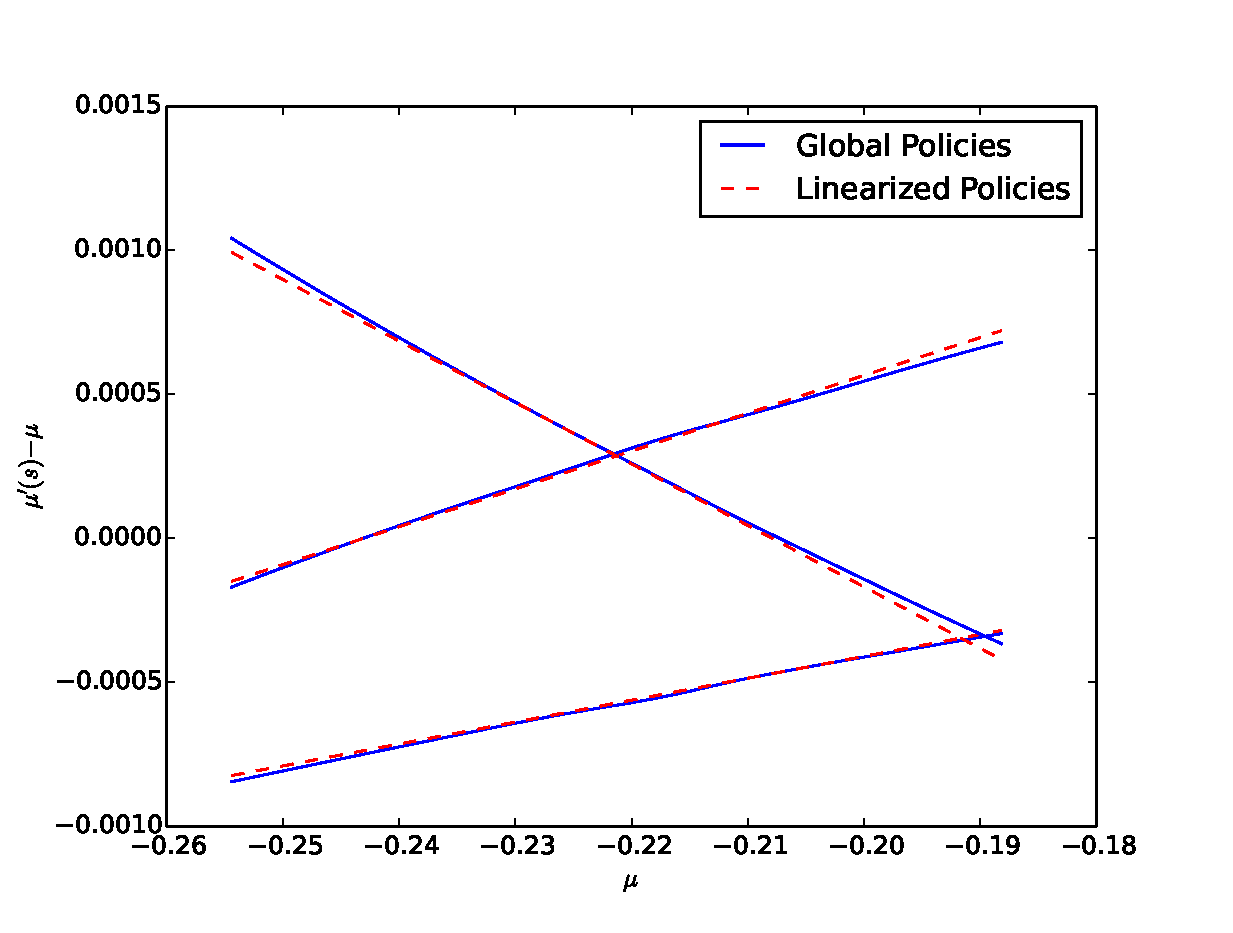
\includegraphics[width=3.5in]{Images/pol1.eps}
	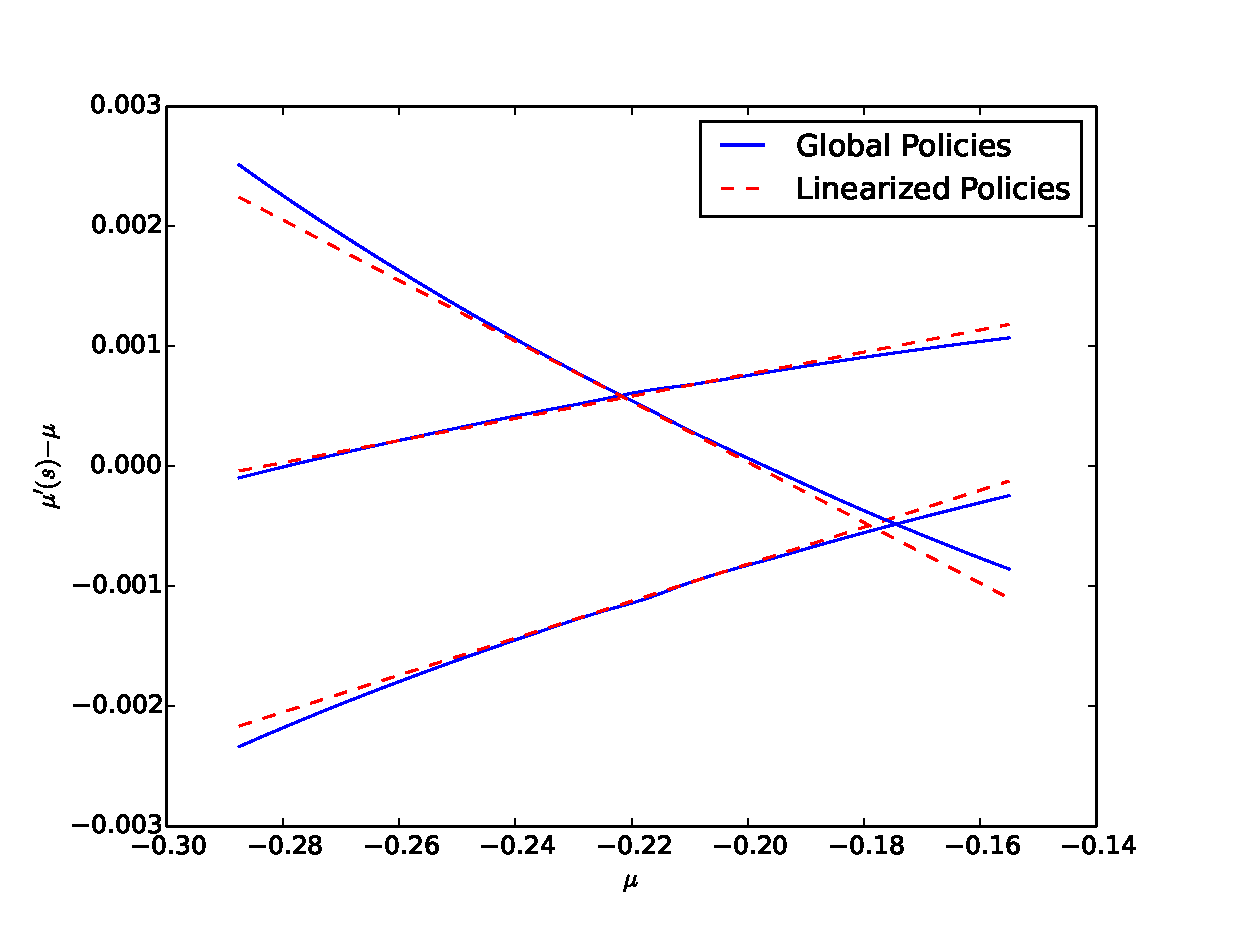
\includegraphics[width=3.5in]{Images/pl2.eps}
	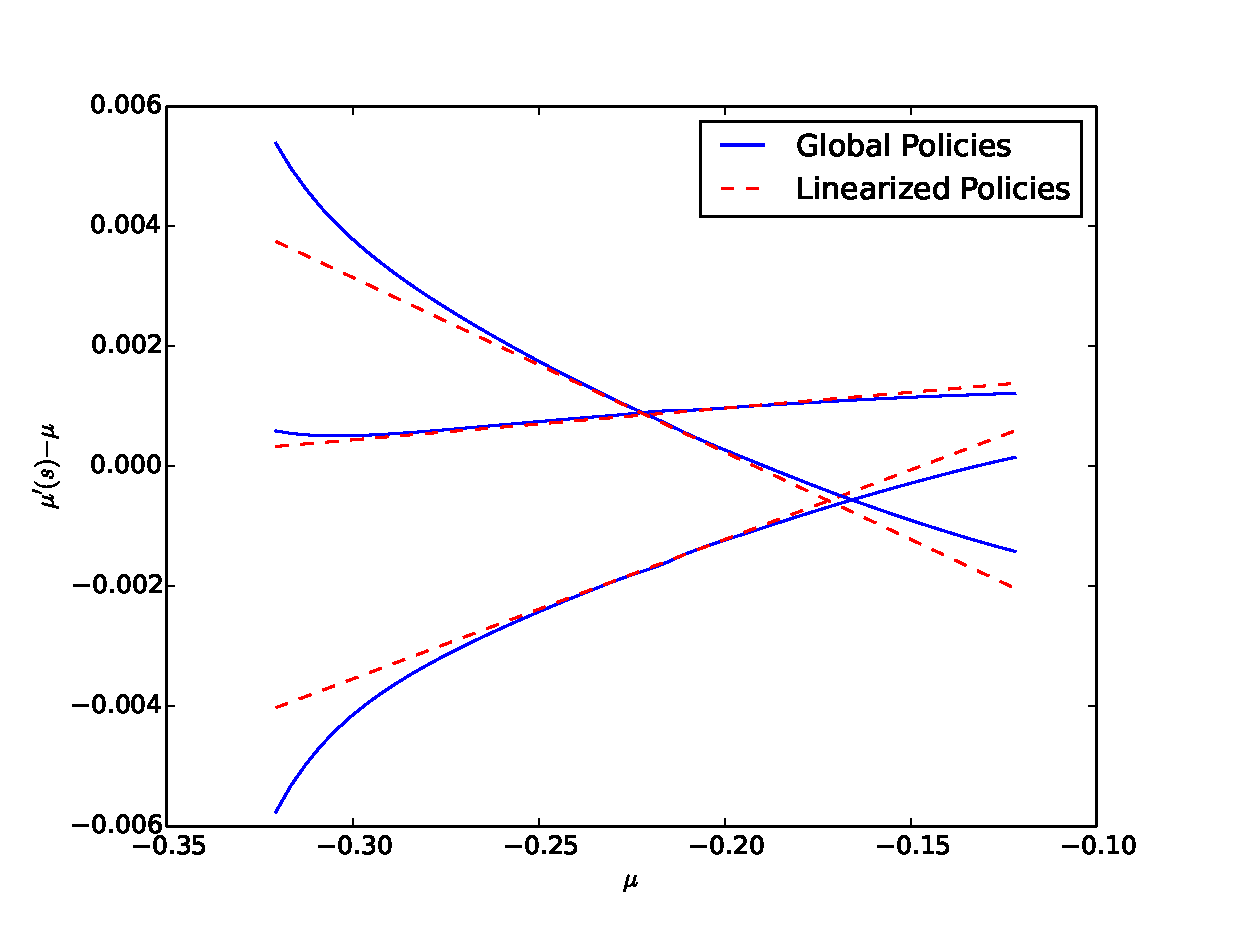
\includegraphics[width=3.5in]{Images/pol3.eps}
	\caption{Policy rules for $\mu'(s)-\mu$ vs $\mu$ for the 3 economies for a range of $\mu$ within $2$ standard devations of the mean.\label{fig.pol_plot}}
\end{figure}

\section{Second Order}
Still a work in progress
\subsection{Computing $\frac{\partial^2 \mu'(s)}{\partial\mu\partial p_s}$}
Taking cross derivatives we quickly obtain
\begin{equation}\label{eq.dimp_dpdmu}
	\frac{\partial^2 b}{\partial\mu\partial p_s}\frac{\pbar_{s'}}{\beta}+\frac{\partial b}{\partial \mu}\frac1\beta\left(1_{s,s'} - \Pi_s \pbar_{s'}\right) = \left[I'(\mubar)+\frac{\partial b}{\partial \mu}\right]\frac{\partial^2 \mu'(s')}{\partial\mu\partial p_s} + \left[I''(\mubar) +\frac{\partial^2 b}{\partial\mu^2}\right]\frac{\partial\mu'(s')}{\partial \mu}\frac{\partial \mu'(s')}{\partial p_s}
\end{equation}and 
\begin{equation}\label{eq.dmart_dmudp}
	0 = \sum_{s'}\Pi_{s'}\pbar_{s'}\frac{\partial^2u'(s')}{\partial \mu\partial p_s} + \Pi_s\left(\frac{\partial\mu'(s)}{\partial\mu}-1\right)
\end{equation}  In order to solve this we need to find  $\frac{\partial ^2 b}{\partial \mu^2}$.  This is done by computing the second derivatives of the first order conditions
\[
	\frac{\partial^2 b}{\partial\mu^2} \frac{\pbar_s}{\beta} =\left[ I'(\mubar) +\frac{\partial b}{\partial\mu}\right]\frac{\partial^2\mu'(s)}{\partial\mu^2} + \left[I''(\mubar)+\frac{\partial^2b}{\partial\mu^2}\right]\left(\frac{\partial \mu'(s)}{\partial\mu}\right)^2
\]and
\[
 0 = \sum_{s'}\Pi_{s'}\pbar_{s'}\frac{\partial^2\mu'(s)}{\partial\mu^2}
\]Combining these to we have
\[
	\frac{\partial^2 b}{\partial \mu^2} \frac{\EE\pbar^2}{\beta} = \left[I''(\mubar)+\frac{\partial^2b}{\partial \mu^2}\right]\frac{\EE\pbar^3}{(\EE\pbar^2)^2}
\]so
\[
	\frac{\partial^2b}{\partial\mu^2} = \frac{\beta I''(\mubar)\EE\pbar^3}{(\EE\pbar^2)^2-\beta\EE\pbar^3}
\]Combining equations \eqref{eq.dimp_dpdmu} and \eqref{eq.dmart_dmudp} we see
\[
	\frac{\EE \pbar^2}{\beta}\frac{\partial^2 b}{\partial\mu\partial p_s} + \frac{\partial b}{\partial \mu}\frac{\Pi_s}\beta(\pbar_s-\EE\pbar^2) = \Pi_s\left[I'(\mubar)+\frac{\partial b}{\partial \mu}\right]\left(1-\frac{\partial \mu'(s)}{\partial \mu}\right)+\left[I''(\mubar)+\frac{\partial^2b}{\partial\mu^2}\right]\EE\left[\pbar\frac{\partial \mu'}{\partial\mu}\frac{\partial\mu'}{\partial p_s}\right]
\]where
\[
\begin{split}
	\EE\left[\pbar\frac{\partial\mu'}{\partial\mu}\frac{\partial \mu'}{\partial p_s}\right]
	&=\sum_{s'}\Pi_{s'}\pbar_{s'}\frac{\pbar_{s'}}{\EE\pbar^2}\frac{\bbar}{\beta\left[I'(\mubar)+\frac{\partial b}{\partial\mu}\right]}\left(1_{s,s'}-\frac{\Pi_s\pbar_s\pbar_{s'}}{\EE\pbar^2}\right)\\
	&=\frac{\bbar}{\beta\EE\pbar^2\left[I'(\mubar)+\frac{\partial b}{\partial \mu}\right]}\left(\Pi_s\pbar_s^2-\Pi_s\pbar_s\frac{\EE\pbar^3}{\EE\pbar^2}\right)\\
	&=\frac{\bbar\Pi_s\pbar_s\left(\pbar_s -\frac{\EE\pbar^3}{\EE\pbar^2}\right)}{\beta\EE\pbar^2\left[I'(\mubar)-\frac{\partial b}{\partial\mu}\right]}
\end{split}
\]Thus 
\begin{equation}
	\frac{\partial^2 b}{\partial \mu\partial p_s} = \Pi_s\left(1-\frac{\pbar_s}{\EE\pbar^2}\right)\frac{\partial b}{\partial \mu} + \Pi_s\left[I'(\mubar)+\frac{\partial b}{\partial \mu}\right]\frac{\EE\pbar^2-\pbar_s}{(\EE\pbar^2)^2}+\Pi_s\left[I''(\mubar)\frac{\partial^2b}{\partial\mu^2}\right]\frac{\bbar\pbar_s\left(\pbar_s-\frac{\EE\pbar^3}{\EE\pbar^2}\right)}{(\EE\pbar^2)^2\left[I'(\mubar)-\frac{\partial b}{\partial\mu}\right]}
\end{equation}and 
\begin{equation}
	\frac{\partial^2\mu'(s)}{\partial\mu\partial p_s}= ...
\end{equation}
\end{document}  



















